\section{Moment Closure Problem and Isotropic Closure}
\label{sec:moment_closure}

The diffusion approximation theories are derived from truncating the moment expansion of the RTE after its first moment and eliminating the unknown $\vec{E}$ by inserting the first moment equations into the zero moment equation, to arrive at a single partial differential equation, which contains the zero moment $\phi$ and the second moment $P$ of the radiance field as unknowns. In order to be able to solve this partial differential equation for $\phi$, it has to be closed by eliminating the second moment $P$ as an unknown. Finding or making an educated guess for the closure $P$ is called the moment closure problem. In this section, we will outline the closure for the classical diffusion approximation and revise it in chapter~\ref{sec:fld} to introduce more sophisticated closures.

When trying to establish an educated guess for $P$, there is some information available that could be used, namely the lower moments. The zero moment $\phi$ expresses the power at $\vec{x}$. That is, the total amount of energy arriving from all directions. With that, the radiance field can be factorized into the total power $\phi$, and its distribution over solid angle $\hat{L}$:
\begin{align*}
L(\vec{x}, \vec{\omega}) = \hat{L}(\vec{x}, \vec{\omega})\phi(\vec{x})
\end{align*}

The total power $\phi$ is an unknown, which shall not be eliminated. Therefore, an educated guess for how this power is distributed over solid angle will be made. This is given by the normalized radiance field $\hat{L}$. It is a probability distribution and its first moment is called the normalized flux $\widehat{\vec{E}}$ which is important with more advanced diffusion theories:
\begin{align*}
\widehat{\vec{E}}(\vec{x}) = \hat{L}_1(\vec{x}) = \int_{\Omega}\frac{L(\vec{x}, \vec{\omega})}{\phi(\vec{x})}\vec{\omega}\ud\vec{\omega} = \frac{1}{\phi(\vec{x})}\int_{\Omega}L(\vec{x}, \vec{\omega})\vec{\omega}\ud\vec{\omega} = \frac{\vec{E}(\vec{x})}{\phi(\vec{x})}
\end{align*}
Seperating the radiance field into power and its distribution over solid angle, allows us to factorize its second moment, the unknown $P$, in the same fashion:
\begin{align*}
P(\vec{x}) &=
\int_{\Omega}{\hat{L}(\vec{x}, \vec{\omega})\phi(\vec{x})N_2\ud\vec{\omega}}\\
&= \int_{\Omega}{\hat{L}(\vec{x}, \vec{\omega})N_2\ud\vec{\omega}}\phi(\vec{x})\\
&= \hat{L}_2(\vec{x}, \vec{\omega})\phi(\vec{x})
\end{align*}
The second moment of the radiance field is expressed as the second moment of the angular radiance distribution, multiplied by the power $\phi$ at $\vec{x}$. This means, that finding a closure at the end results in finding or estimating a spherical distribution function. The second moment of that estimated distribution is called the Eddington tensor~$T$:
\begin{align}
\label{eq:eddington_tensor}
T(\vec{x}) \approx \hat{L}_2(\vec{x}, \vec{\omega}) =
\frac{P(\vec{x})}{\phi(\vec{x})} =
\widehat{P}(\vec{x})
\end{align}
The Eddington tensor is used to distribute the known power $\phi$ over angle and approximate $P$:
\begin{align*}
T(\vec{x})\phi(\vec{x}) \approx 
P(\vec{x})
\end{align*}
The key assumption behind the classical diffusion approximation is that the radiance field $L$ is constant and does not change for different angles $\vec{\omega}$:
\begin{align*}
L(\vec{x}, \vec{\omega}) = L(\vec{x})
\end{align*}
This assumption allows for finding an estimate $T$ for the second moment of the radiance distribution. Unit power $\phi = 1$ is assumed:
\begin{align*}
1 = \phi\left(\vec{x}\right) = \int_\Omega{L\left(\vec{x}, \vec{\omega}\right)\ud\vec{\omega}}
\end{align*}
Since $L$ is constant over solid angle ($L(\vec{x}, \vec{\omega})=L(\vec{x})$), it can be extracted out of the integral to get:
\begin{align*}
1 = \phi\left(\vec{x}\right) = L\left(\vec{x}\right)\int_\Omega{\ud\vec{\omega}}\implies L\left(\vec{x}\right) = \frac{1}{4\pi}
\end{align*}
The constant radiance field is used to compute the components of the radiative pressure tensor:
\begin{align*}
P\left(\vec{x}\right) 
= \int_\Omega{L\left(\vec{x}\right)N_2\ud\vec{\omega}}
= \frac{1}{4\pi}\int_\Omega{N_2\ud\vec{\omega}}
= \frac{1}{4\pi}\frac{4\pi}{3}\mathbf{I}
= \frac{1}{3}\mathbf{I}
\end{align*}
Since the unit power $\phi(\vec{x})=1$ was assumed without loss of generality, the result is:
\begin{align*}
T(\vec{x})\phi(\vec{x}) = P(\vec{x}) \implies T(\vec{x})=\frac{1}{3}\mathbf{I}
\end{align*}
Inserting $P=T\phi=\frac{1}{3}\mathbf{I}\phi$ into equation~\ref{eq:general_diffusion_equation}, gives the diffusion equation for anisotropic emission sources
\begin{align}
\label{eq:diffusion_equation_anisotropic_Q}
\nabla
\left(
-\frac{1}{3\sigma_t'\left(\vec{x}\right)}
\nabla \phi\left(\vec{x}\right)
\right)&=
-\phi(\vec{x})\sigma_a(\vec{x})
+Q_0\left(\vec{x}\right)
+\nabla Q_1\left(\vec{x}\right)
\end{align}
and becomes the popular diffusion approximation formula for isotropic emission sources ($Q_1=\vec{0}$):
\begin{align}
\label{eq:diffusion_equation_anisotropic_Q}
\nabla
\left(
D
\nabla \phi\left(\vec{x}\right)
\right)&=
-\phi(\vec{x})\sigma_a(\vec{x})
+Q_0\left(\vec{x}\right)
\end{align}
with the classic linear diffusion coefficient
\begin{align}
D=-\frac{1}{3\sigma_t'\left(\vec{x}\right)}
.
\label{eq:da_D}
\end{align}
Inserting the isotropic second moment into the first moment expansion of the radiative transfer equation (equation~\ref{eq:me_first_resolved_E}) gives an expression for the flux-vector, as defined by the diffusion approximation theory:
\begin{align}
\label{eq:diffusion_ficks_law}
\vec{E}\left(\vec{x}\right) \approx -D\left(\vec{x}\right)\nabla\phi\left(\vec{x}\right)
\end{align}
This allows for some intuition about the diffusion approximation. Instead of depending on the global radiance field $L$, the flux-vector depends on the local gradient of the fluence to determine the transport of radiative energy at position $\vec{x}$.
\begin{figure}[h]
\centering
%\missingfigure{Visualize the idea behind diffusion approximation: to approximate global transport by using a local gradient of the fluence. mention ficks law of diffusion}
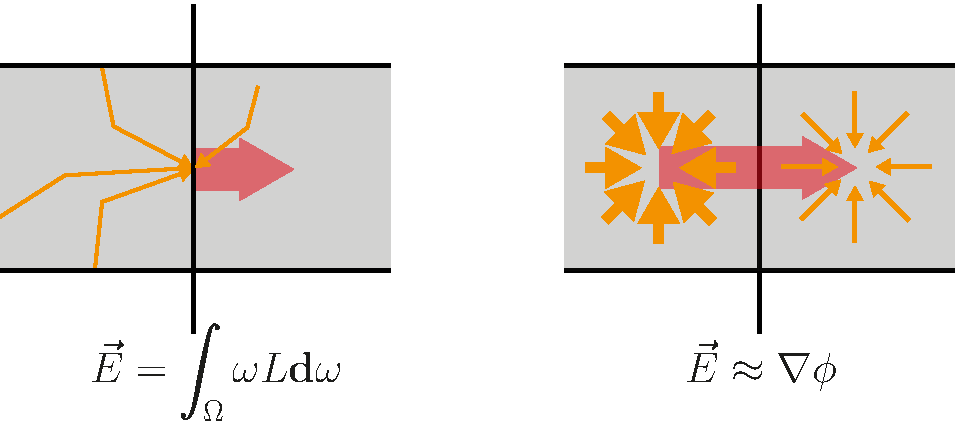
\includegraphics[width=0.85\textwidth]{05_diffusion_approximation/figures/fig_diffusion_idea.pdf}
\caption{Ficks first law of diffusion (visualized on the right) states that the diffusive flux can be related to the difference in concentration (of fluence $\phi$), allowing to approximate a global quantity (left) by a local quantity. This is the fundamental idea behind diffusion approximation.}
\label{fig:da_moment_problem_flux_as_fluence_gradient}
\end{figure}
The problem is now uniquely defined and can be solved with standard solvers. In the next section, we discuss how results from diffusion approximation compare against the results from the $P_N$-method.
